\section{Additional Ablation Study}
\label{appendix:training_ablations}

While the main experiments demonstrate the effectiveness of Cosmos 3 across a wide range of understanding and generation tasks, they do not fully isolate the contributions of individual design choices. To better understand the factors underlying the model's capabilities, we conduct a series of ablation studies examining key architectural, data, and training decisions. These studies investigate how the Reasoner and Generator interact within the Mixture-of-Transformers framework, the impact of multimodal training signals such as audio and action data, the effectiveness of temporal conditioning mechanisms, and the transferability of learned world and action representations across domains. Together, these analyses provide deeper insight into the design principles that enable Cosmos 3 to function as a unified omnimodal world model for Physical AI.s

\subsection{How the Reasoner Benefits the Generator}
In this study, we investigate how the Reasoner benefits the Generator model. We train two models using the Cosmos3-Nano architecture: one with Qwen3-VL-8B as the understanding tower, and the other with our Cosmos3-Nano Reasoner. In both cases, the Generator tower is trained from scratch. For this ablation, we restrict training to 256p and 480p resolutions with clip lengths of 0–200 frames, and set the sequence length to 25K. Following our large-scale run, we use joint image–video training. Both models are trained for 90K iterations on 256 GPUs. We report PAIBench scores for both below.

\newcommand{\roth}[1]{\rotatebox[origin=l]{90}{\small #1}}

\newcommand{\vraise}[1]{\raisebox{3.0em}{#1}}

\begin{table}[h]
\centering
\caption{\textbf{Understanding tower ablation.} We report domain and quality scores on PAIBench T2V and I2V for two variants that differ only in the pretrained model used to initialize the understanding tower while the Generator tower is trained from scratch: (1) Cosmos 3 Reasoner and (2) Qwen3-VL. Subject and background consistency are I2V-specific and not applicable to T2V. Initializing the understanding tower from the Cosmos3 Reasoner yields better domain scores on Physical AI domains than the Qwen3-VL variant.}
\setlength{\tabcolsep}{4pt}
\renewcommand{\arraystretch}{1.15}
\resizebox{\linewidth}{!}{%
\begin{tabular}{@{}ll | ccc | cccccc | cccccc | cc@{}}
\toprule
\multicolumn{2}{c}{} & \multicolumn{3}{c}{\textbf{Summary}} & \multicolumn{6}{c}{\textbf{Domain}} & \multicolumn{6}{c}{\textbf{Quality}} & \multicolumn{2}{c}{\textbf{I2V}} \\
\cmidrule(lr){3-5} \cmidrule(lr){6-11} \cmidrule(lr){12-17} \cmidrule(lr){18-19}
\textbf{Bench} & \textbf{Und. tower}
 & Overall & Domain & Quality
 & C.S. & AV & Rob. & Ind. & Hum. & Phy.
 & Subj. & Bg. & Motion & Aesth. & Imag. & Cons.
 & Subj. & Bg. \\
\midrule
\multirow{2}{*}{T2V}
& \cellcolor{rowours}Cosmos3 Reasoner  & \cellcolor{rowours}\textbf{74.3} & \cellcolor{rowours}\textbf{75.7} & \cellcolor{rowours}73.0          & \cellcolor{rowours}\textbf{81.2} & \cellcolor{rowours}\textbf{54.9} & \cellcolor{rowours}\textbf{71.3} & \cellcolor{rowours}\textbf{78.4} & \cellcolor{rowours}\textbf{76.2} & \cellcolor{rowours}\textbf{89.2} & \cellcolor{rowours}\textbf{96.0} & \cellcolor{rowours}\textbf{96.8} & \cellcolor{rowours}99.4          & \cellcolor{rowours}\textbf{55.2} & \cellcolor{rowours}71.4          & \cellcolor{rowours}\textbf{19.1} & \cellcolor{rowours}--            & \cellcolor{rowours}--            \\
& Qwen-3 VL & 73.3          & 73.7          & \textbf{73.0} & 80.5          & 52.6          & 66.5          & 77.4          & 74.0          & 88.7          & 95.8          & 96.6          & \textbf{99.4} & 55.0          & \textbf{72.2} & 19.0          & --            & --            \\
\midrule
\multirow{2}{*}{I2V}
& \cellcolor{rowours}Cosmos3 Reasoner  & \cellcolor{rowours}\textbf{79.4} & \cellcolor{rowours}\textbf{80.8} & \cellcolor{rowours}\textbf{78.1} & \cellcolor{rowours}89.0          & \cellcolor{rowours}59.4          & \cellcolor{rowours}\textbf{77.0} & \cellcolor{rowours}\textbf{84.8} & \cellcolor{rowours}\textbf{79.3} & \cellcolor{rowours}\textbf{91.6} & \cellcolor{rowours}\textbf{92.4} & \cellcolor{rowours}\textbf{94.7} & \cellcolor{rowours}99.4          & \cellcolor{rowours}\textbf{53.2} & \cellcolor{rowours}68.7          & \cellcolor{rowours}\textbf{20.2} & \cellcolor{rowours}\textbf{98.0} & \cellcolor{rowours}\textbf{98.0} \\
& Qwen-3 VL & 79.0          & 80.0          & 78.0          & \textbf{89.7} & \textbf{59.8} & 74.0          & 84.0          & 78.3          & 91.4          & 92.0          & 94.5          & \textbf{99.4} & 53.1          & \textbf{69.3} & 20.1          & 97.9          & 97.9          \\
\bottomrule
\end{tabular}%
}
\label{tab::ablation-understanding-tower}
\end{table}

As shown in Table~\ref{tab::ablation-understanding-tower}, replacing Qwen3-VL-8B with our Cosmos3-Nano Reasoner in the understanding tower yields consistent improvements in domain scores, particularly in Physical AI domains. On T2V, the Reasoner improves the overall Domain score from 73.7 to 75.7, with the largest gains concentrated in physically-grounded categories: Robot (+4.8, 66.5 → 71.3), Physics (+0.5, 88.7 → 89.2), AV (+2.3, 52.6 → 54.9), and Industry (+1.0, 77.4 → 78.4). A similar pattern holds on I2V, where the Domain score rises from 80.0 to 80.8, driven by gains in Common sense (+0.7), Industry (+0.8), Human (+1.0), and Physics (+0.2). These results suggest that the reasoner provides better embeddings for Physical AI domains for generator to learn. The quality scores for both models are comparable.

\subsection{Choice of FPS Control}

We study two complementary mechanisms for conditioning generation on a target frame rate: (i) MRoPE FPS modulation, which scales the temporal axis of the unified 3D MRoPE by the target FPS, and (ii) Text Control, which injects the target duration and FPS as natural-language text inside the structured JSON caption. For this ablation, we
restrict training to 256p and 480p resolutions with clip lengths of 0–200 frames, and set the sequence length
to 25K. Following our large-scale run, we use joint image–video training. We train 4 models for 130K iterations on 128 GPUs each, varying only whether each mechanism is active: Base (no control), Text Control (text only), MRoPE FPS Modulation (MRoPE only), and Text Control + MRoPE FPS Modulation (both). We curate an evaluation set with known source duration and FPS, $\sim$100 videos each of 10, 15, 24, 30 FPS ($\pm$2 FPS tolerance). We use the structured captions of these evaluation set videos as prompts and generate samples across 3 seeds per prompt at 480p (16:9) resolution. We produce a 5 s clip for each prompt.

We score each clip on Video Quality (VQ; DOVER perceptual quality score~\citep{dover}) and Dynamic Degree (DD; motion presence on a 0--1 scale~\citep{huang2023vbench}). From the three-seed DD scores per prompt ($p$), we compute a normalized motion control (MC) term
\begin{equation}
    \text{MC} = \mathbb{E}_{p}\!\left[\frac{\text{var}_p}{\text{var}_p + \text{mean}_p^2}\right],
\end{equation}
MC indicates the robustness of the control mechanism, \ie, the degree of variability per prompt for each control setting. We combine these into a Motion Fidelity score
\begin{equation}
    \text{MF} = (1 - |\text{DD} - \text{DD}_{\text{ref}}|)\,(1 - \text{MC}),
\end{equation}
where $\text{DD}_{\text{ref}}$ is the per-band mean DD over the real-video reference set. The final Composite Score is the product of Video Quality and Motion Fidelity, reflecting adherence to motion magnitude without impacting the perceptual quality of generated videos. This is computed as $\mathbb{E}_{\text{FPS-band}}\!\left[(\text{VQ}) \cdot \text{MF}\right]$, computed per FPS band and then averaged across bands.

\cref{tab:fps_control_ablation} reports averages across the four FPS bands. Both mechanisms improve over Base individually; MRoPE FPS modulation alone yields a larger gain than the Text Control ($+1.12$ vs.\ $+0.77$ in composite). Combining the two produces the best composite score ($+1.30$ over Base). VQ stays within a 0.2-point window across all four settings, indicating that the gains are concentrated in motion fidelity rather than video perceptual quality, \ie, the controls primarily improve temporal behavior. Based on these results, we adopt the Text Control + MRoPE FPS Modulation configuration for Cosmos 3 Generator.

\begin{table}[h]
\label{tab::fps_control}
    \centering
    \captionsetup{justification=raggedright, singlelinecheck=false}
    \caption{\textbf{FPS control ablation on Cosmos3-Nano.} Scores are averaged across four FPS bands (10, 15, 24, 30). VQ is the DOVER video quality score; MF is motion fidelity (0--1); Composite $= \mathbb{E}_{\text{band}}[(\text{VQ}) \cdot \text{MF}]$. \textbf{Bold} indicates best in the column. Text Control + MRoPE FPS Modulation is the most performant control setting that demonstrates adherence to reference FPS band motion while preserving perceptual quality.}
    \label{tab:fps_control_ablation}
    \setlength{\tabcolsep}{8pt}
    \renewcommand{\arraystretch}{1.25}
    \resizebox{\linewidth}{!}{
    \begin{tabular}{l l c c c}
        \toprule
        \textbf{Model} & \textbf{FPS Control Setting} & \textbf{Avg.\ VQ ($\uparrow$)} & \textbf{Avg.\ MF ($\uparrow$)} & \textbf{Avg.\ Composite ($\uparrow$)} \\
        \midrule
        Cosmos3-Nano & Base (No Control)  & 12.89 & 0.6626 & 8.51 \\
        Cosmos3-Nano & Text Control            & 12.99 & 0.7169 & 9.28 \\
        Cosmos3-Nano & MRoPE FPS Modulation & \textbf{13.03} & 0.7409 & 9.63 \\
        % \rowcolor{rowours}
        Cosmos3-Nano & \textbf{Text Control + MRoPE FPS Modulation} & 12.84 & \textbf{0.7649} & \textbf{9.81} \\
        \bottomrule
    \end{tabular}
    }
\end{table}

\subsection{Audio Data in Pre-Training}

We investigate the impact of including audio during continued pre-training on video metrics. Starting from the same pre-trained checkpoint, we train two Cosmos3-Nano variants on our pre-training dataset: one with video-only data and one with joint video-audio data. These ablations are run for 20k iterations on 128 GPUs. We restrict training to 256p and 480p resolutions.

\begin{table}[h]
\centering
\caption{\textbf{Effect of introducing audio data during pre-training.} We report PAIBench T2V and I2V scores after continued pre-training of two generator variants that differ only in whether audio is used during training. The video data is shared across both experiments.}
\setlength{\tabcolsep}{4pt}
\renewcommand{\arraystretch}{1.15}
\resizebox{\linewidth}{!}{%
\begin{tabular}{@{}ll | ccc | cccccc | cccccc | cc@{}}
\toprule
\multicolumn{2}{c}{} & \multicolumn{3}{c}{\textbf{Summary}} & \multicolumn{6}{c}{\textbf{Domain}} & \multicolumn{6}{c}{\textbf{Quality}} & \multicolumn{2}{c}{\textbf{I2V}} \\
\cmidrule(lr){3-5} \cmidrule(lr){6-11} \cmidrule(lr){12-17} \cmidrule(lr){18-19}
\textbf{Bench} & \textbf{Variant}
 & Overall & Domain & Quality
 & C.S. & AV & Rob. & Ind. & Hum. & Phy.
 & Subj. & Bg. & Motion & Aesth. & Imag. & Cons.
 & Subj. & Bg. \\
\midrule
\multirow{2}{*}{T2V} & Without Audio  & 78.6 & 83.8 & \textbf{73.4} & 90.7 & 64.7 & 81.9 & 84.4 & 82.7 & \textbf{94.8} & \textbf{95.9} & \textbf{97.1} & \textbf{99.5} & \textbf{57.3} & \textbf{70.6} & 19.8 & -- & -- \\
 & \cellcolor{rowours}With Audio  & \cellcolor{rowours}\textbf{79.1} & \cellcolor{rowours}\textbf{85.0} & \cellcolor{rowours}73.2 & \cellcolor{rowours}\textbf{91.5} & \cellcolor{rowours}\textbf{67.9} & \cellcolor{rowours}\textbf{83.8} & \cellcolor{rowours}\textbf{86.1} & \cellcolor{rowours}\textbf{83.7} & \cellcolor{rowours}93.8 & \cellcolor{rowours}95.5 & \cellcolor{rowours}96.9 & \cellcolor{rowours}\textbf{99.5} & \cellcolor{rowours}57.1 & \cellcolor{rowours}70.2 & \cellcolor{rowours}\textbf{19.9} & \cellcolor{rowours}-- & \cellcolor{rowours}-- \\
\midrule
\multirow{2}{*}{I2V} & Without Audio  & 81.7 & 85.1 & \textbf{78.4} & 93.2 & 67.5 & 82.0 & 86.0 & 83.2 & \textbf{95.1} & \textbf{93.3} & \textbf{95.1} & \textbf{99.5} & \textbf{55.0} & 67.6 & \textbf{20.4} & \textbf{98.4} & \textbf{98.3} \\
 & \cellcolor{rowours}With Audio  & \cellcolor{rowours}\textbf{82.2} & \cellcolor{rowours}\textbf{85.9} & \cellcolor{rowours}\textbf{78.4} & \cellcolor{rowours}\textbf{93.6} & \cellcolor{rowours}\textbf{68.6} & \cellcolor{rowours}\textbf{84.2} & \cellcolor{rowours}\textbf{86.5} & \cellcolor{rowours}\textbf{84.3} & \cellcolor{rowours}94.8 & \cellcolor{rowours}92.9 & \cellcolor{rowours}94.9 & \cellcolor{rowours}99.4 & \cellcolor{rowours}\textbf{55.0} & \cellcolor{rowours}\textbf{67.9} & \cellcolor{rowours}\textbf{20.4} & \cellcolor{rowours}98.2 & \cellcolor{rowours}98.2 \\
\bottomrule
\end{tabular}%
}
\label{tab::ablation-audio-pretraining}
\end{table}

The results in~\cref{tab::ablation-audio-pretraining} show that continued training without audio leads to a drop in both T2V and I2V scores, suggesting that joint video-audio pre-training does not degrade video generation quality and may provide a modest benefit even when evaluated purely on video-centric metrics.

\subsection{Synergy Between Action Modes}
\label{app:pusht_fd_id_policy_synergy}
As described in \cref{sec::generation_mode_def} and summarized in \cref{fig:action_modes}, Cosmos 3 supports three action generation modes: forward dynamics (FD), inverse dynamics (ID), and joint video-action prediction (policy).
We ablate whether a single joint action model can share useful structure across these modes.
We use the PushT dataset and Cosmos3-Edge for this experiment.
The model is trained for three single-mode action checkpoints for 2K steps each against one joint FD/ID/policy checkpoint trained for 6K steps, so that each mode is trained for the same amount of optimization steps.
We report the PSNR for FD and MSE for ID.
For policy mode, we report the policy coverage ratio of the T block and target region aggregated across 50 different initializations, with 10 rollouts from each starting point.
The results are summarized in \cref{tab:pusht_fd_id_policy_open_loop}.

\begin{table}[h]
\centering
\caption{\textbf{PushT action-mode synergy.} We compare single-mode FD, ID, and policy checkpoints trained for 2K steps each against one joint FD/ID/policy checkpoint trained for 6K steps. Lower is better for ID MSE; higher is better for FD PSNR and policy coverage. \textbf{Bold} indicates the better value in each column.}
\label{tab:pusht_fd_id_policy_open_loop}
\small
\setlength{\tabcolsep}{7pt}
\renewcommand{\arraystretch}{1.15}
\begin{tabular}{@{}lccc@{}}
\toprule
\textbf{Training setting} & \textbf{FD PSNR $\uparrow$} & \textbf{ID MSE $\downarrow$} & \textbf{Policy Coverage $\uparrow$} \\
\midrule
2K single-mode & \textbf{27.13} & $1.11 \times 10^{-3}$ & 74.1\% \\
6K joint FD/ID/policy & 26.22 & $\boldsymbol{3.09 \times 10^{-4}}$ & \textbf{77.3\%} \\
\bottomrule
\end{tabular}
\end{table}


The joint FD/ID/policy checkpoint improves the action-side metrics while preserving comparable forward-dynamics quality.
Compared with the single-mode checkpoints, ID MSE decreases from $1.11 \times 10^{-3}$ to $3.09 \times 10^{-4}$, a 72\% relative reduction, and policy coverage increases from 74.1\% to 77.3\%.
FD PSNR decreases from 27.13 to 26.22, indicating a modest tradeoff in reconstruction fidelity.
Overall, the joint checkpoint provides the best policy coverage and ID accuracy under the same per-mode optimization budget, suggesting that the action modes share useful structure even though FD quality benefits slightly from single-mode specialization.

\FloatBarrier

\subsection{Video-Action Consistency}
\label{app:robolab_video_action_consistency}
In addition to the closed-loop success rate reported in \cref{sec:robot_manip_policy}, we evaluate how well the video and action streams jointly predicted by Cosmos3-Nano-Policy-DROID remain aligned on RoboLab. 
Cosmos3-Nano-Policy-DROID is trained only on DROID, so RoboLab provides a held-out environment for testing this video-action consistency.
For each predicted action chunk, we execute the same chunk in the RoboLab simulator and compute PSNR between the model-predicted video and the resulting simulator rollout, then aggregate the scores across action chunks for the left and wrist camera views.
The left third-person view achieves 23.19\,dB, comparable to the PSNR levels achieved by our robotics forward-dynamics models on DROID (\cref{tab:action_posttraining_summary_wide}).
The wrist (eye-in-hand) view is more challenging because the camera moves with the end-effector and the model must infer newly revealed content; nevertheless, it reaches 17.33\,dB. 
These results indicate strong consistency between the predicted actions and predicted videos.
\Cref{fig:robolab_video_action_consistency} visualizes this consistency: the predicted frames closely match the corresponding frames from simulator rollouts initialized from the same state.

\begin{figure}[!htbp]
    \centering
    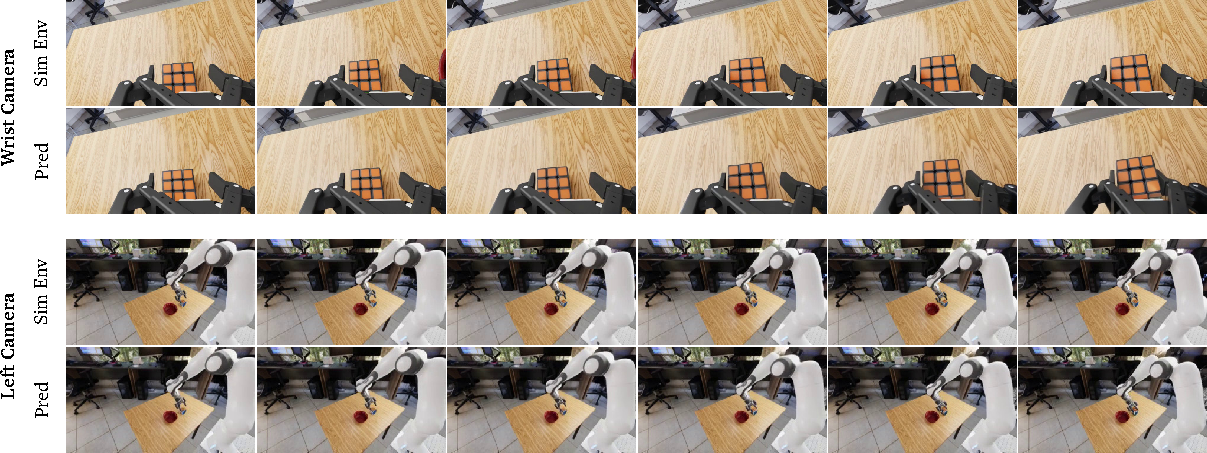
\includegraphics[width=\linewidth]{figures/results/action/consistency/robolab_video_action_consistency_figure.pdf}

    \caption{\textbf{Predicted video vs.\ simulator rollout on RoboLab.} For the wrist and left cameras, \textit{Sim Env} shows the video recorded by executing the predicted action chunk in the RoboLab simulator from the same initial state, while \textit{Pred} shows the video predicted by \textbf{Cosmos3-Nano-Policy-DROID} jointly with that action chunk. We observe that the predicted video closely matches the simulator rollout.}
    \label{fig:robolab_video_action_consistency_rubikscube}
    \label{fig:robolab_video_action_consistency}
\end{figure}

\FloatBarrier
